\section{\numb section 2. Meshes and manifolds}

This section describes several examples of meshes, some of them built on specific manifolds.
Note that in this manual we use the term ``manifold'' to mean a manifold without boundary.

% Paragraphs \numb section 2.\numb parag 1, \numb section 2.\numb parag 2,
% \numb section 2.\numb parag 3, \numb section 2.\numb parag 4, \numb section 2.\numb parag 8,
% \numb section 2.\numb parag 9, \numb section 2.\numb parag 13 and
% \numb section 2.\numb parag 14 show examples of meshes in $ \RR^2 $, while paragraphs
% \numb section 2.\numb parag 5, \numb section 2.\numb parag 6, \numb section 2.\numb parag 7,
% \numb section 2.\numb parag 10, \numb section 2.\numb parag 11, \numb section 2.\numb parag 12,
% \numb section 2.\numb parag 15 and \numb section 2.\numb parag 16 show examples in $ \RR^3 $.
Paragraphs \numb section 2.\numb parag 3, \numb section 2.\numb parag 4,
\numb section 2.\numb parag 8, and \numb section 2.\numb parag 9 deal with one-dimensional
meshes (curves) in $ \RR^2 $,
paragraphs \numb section 2.\numb parag 11, \numb section 2.\numb parag 12,
\numb section 2.\numb parag 13 and \numb section 2.\numb parag 14 show curves in $ \RR^3 $,
paragraphs \numb section 2.\numb parag 1, \numb section 2.\numb parag 2,
\numb section 2.\numb parag 8 and \numb section 2.\numb parag 9 show plane domains
(two-dimensional meshes in $ \RR^2 $),
while paragraphs \numb section 2.\numb parag 5, \numb section 2.\numb parag 6,
\numb section 2.\numb parag 7, \numb section 2.\numb parag 11, \numb section 2.\numb parag 12,
\numb section 2.\numb parag 15 and \numb section 2.\numb parag 16 focus on two-dimensional meshes
in $ \RR^3 $ (surfaces).

Paragraphs \numb section 2.\numb parag 3 -- \numb section 2.\numb parag 12
are about manifolds defined implicitly as level sets; paragraphs \numb section 2.\numb parag 13 --
\numb section 2.\numb parag 16 describe parametric manifolds.

% Paragraphs \numb section 2.\numb parag 1 -- \numb section 2.\numb parag 12 are about building
% meshes of regular shape and them joining them together like patches, while paragraps
% \numb section 2.\numb parag 13 -- \dots show
% how to directly mesh a domain starting from its boundary only.


\paragraph{\numb section 2.\numb parag 1. Joining segments}

Here is another way of meshing the same L-shaped domain as in paragraph
\numb section 1.\numb parag 3 :

{ \psfrag{A}{\special{ps: gsave 0 0 0.8 setrgbcolor}{\codett A}\special{ps: grestore}}
\psfrag{B}{}
\psfrag{C}{\special{ps: gsave 0 0 0.8 setrgbcolor}{\codett C}\special{ps: grestore}}
\psfrag{D}{\special{ps: gsave 0 0 0.8 setrgbcolor}{\codett D}\special{ps: grestore}}
\psfrag{E}{\special{ps: gsave 0 0 0.8 setrgbcolor}{\codett E}\special{ps: grestore}}
\psfrag{F}{\special{ps: gsave 0 0 0.8 setrgbcolor}{\codett F}\special{ps: grestore}}
\psfrag{G}{\special{ps: gsave 0 0 0.8 setrgbcolor}{\codett G}\special{ps: grestore}}
\psfrag{H}{\special{ps: gsave 0 0 0.8 setrgbcolor}{\codett H}\special{ps: grestore}}
\centerline{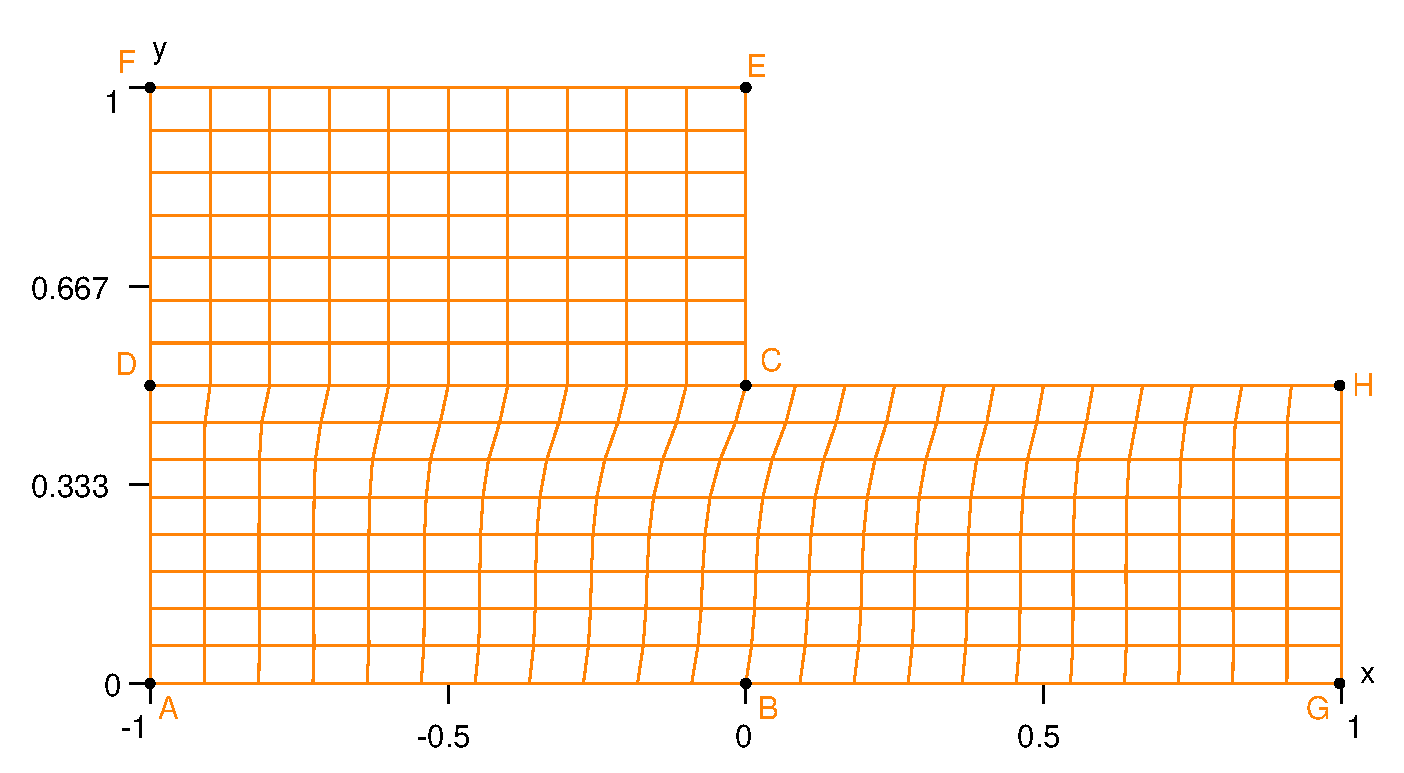
\includegraphics[width=90mm]{L-shaped-distorted.eps}} }

\verbatim
   Mesh AG ( tag::segment, A.reverse(), G, tag::divided_in, 22 );
   Mesh GH ( tag::segment, G.reverse(), H, tag::divided_in, 8 );
   Mesh HC ( tag::segment, H.reverse(), C, tag::divided_in, 12 );
   Mesh CD ( tag::segment, C.reverse(), D, tag::divided_in, 10 );
   Mesh HD ( tag::join, HC, CD );
   Mesh DA ( tag::segment, D.reverse(), A, tag::divided_in, 8 );
   Mesh CE ( tag::segment, C.reverse(), E, tag::divided_in, 7 );
   Mesh EF ( tag::segment, E.reverse(), F, tag::divided_in, 10 );
   Mesh FD ( tag::segment, F.reverse(), D, tag::divided_in, 7 );
   Mesh AGHD ( tag::rectangle, AG, GH, HD, DA );
   Mesh CEFD ( tag::rectangle, CE, EF, FD, CD.reverse() );
   Mesh L_shaped ( tag::join, AGHD, CEFD );
\endverbatim

The only difference between this mesh an the one presented in paragraph \numb section 1.\numb parag 3
is a slight distortion in the lower half of the domain,
due to the non-uniform distribution of the vertices along {\codett HD}.

See paragraph \numb section 9.\numb parag 2 for more details about tags.
See also paragraph \numb section 9.\numb parag 7.


\vfil\eject
\paragraph{\numb section 2.\numb parag 2. Triangular meshes on rectangles}

On a rectangular domain, we can build a mesh of triangles by using the {\codett Mesh} constructor
with {\codett tag::rectangle}, providing as last argument the {\codett tag::with\_triangles}.
For instance, in the example \numb section 1.\numb parag 3, if we re-write the definition of
{\codett BGHC} as

\verbatim
   Mesh BGHC ( tag::rectangle, BG, GH, HC, BC.reverse(), tag::with_triangles );
\endverbatim

\noindent we get the mesh shown below.

{ \psfrag{A}{\special{ps: gsave 0 0 0.8 setrgbcolor}{\codett A}\special{ps: grestore}}
\psfrag{B}{\special{ps: gsave 0 0 0.8 setrgbcolor}{\codett B}\special{ps: grestore}}
\psfrag{C}{\special{ps: gsave 0 0 0.8 setrgbcolor}{\codett C}\special{ps: grestore}}
\psfrag{D}{\special{ps: gsave 0 0 0.8 setrgbcolor}{\codett D}\special{ps: grestore}}
\psfrag{E}{\special{ps: gsave 0 0 0.8 setrgbcolor}{\codett E}\special{ps: grestore}}
\psfrag{F}{\special{ps: gsave 0 0 0.8 setrgbcolor}{\codett F}\special{ps: grestore}}
\psfrag{G}{\special{ps: gsave 0 0 0.8 setrgbcolor}{\codett G}\special{ps: grestore}}
\psfrag{H}{\special{ps: gsave 0 0 0.8 setrgbcolor}{\codett H}\special{ps: grestore}}
\centerline{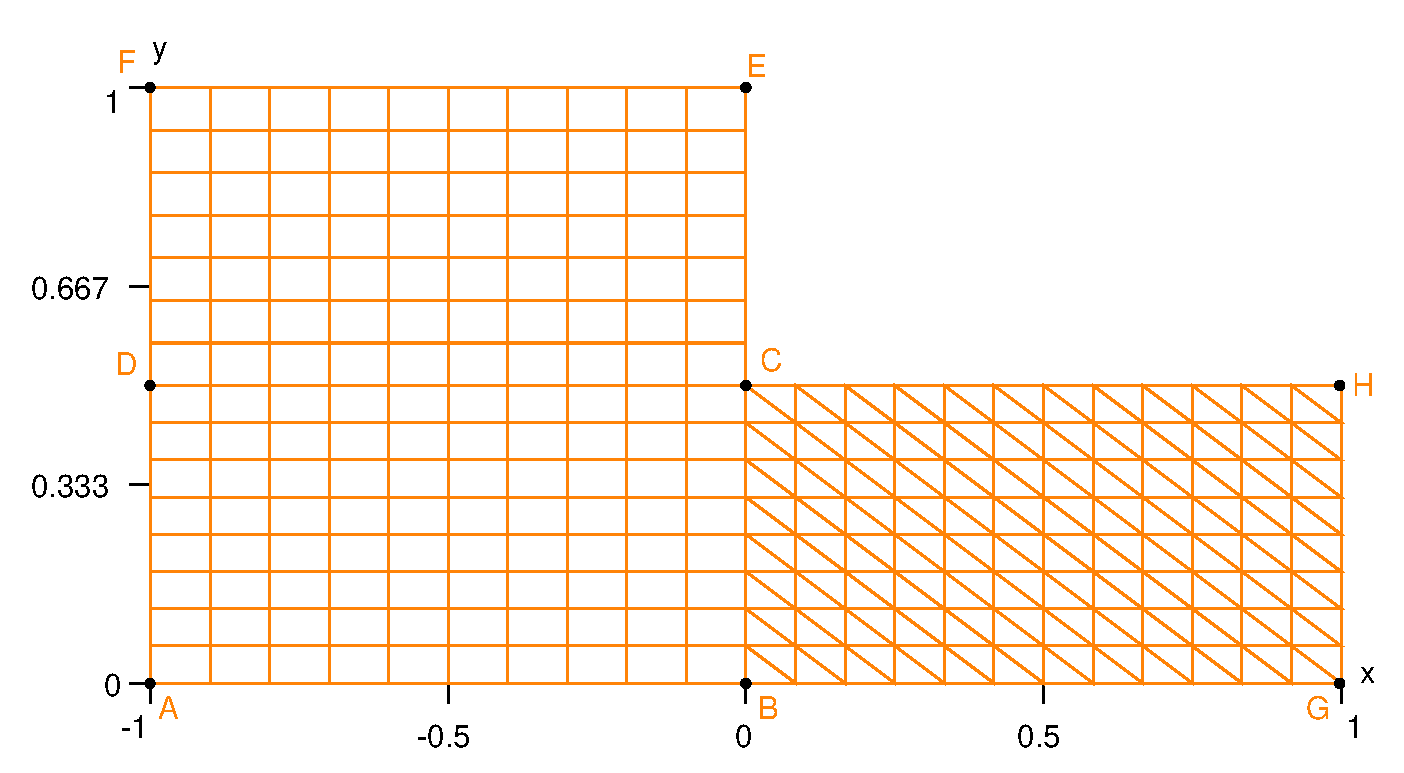
\includegraphics[width=90mm]{L-shaped-tri.eps}} }

If we give the sides of the rectangle in a different order, like in

\verbatim
   Mesh BGHC ( tag::rectangle, GH, HC, BC.reverse(), BG, tag::with_triangles );
\endverbatim

\noindent the rectangles will be cut along the other diagonal (check it yourself).

The mesh in paragraph \numb section 1.\numb parag 4 could have been built like this :

\verbatim
   Mesh ABD ( tag::triangle, AB, BD, AD.reverse() );
   Mesh BCED ( tag::quadrangle, CE, ED, BD.reverse(), BC, tag::with_triangles );
   Mesh one_tri_one_rect ( tag::join, ABD, BCED );
\endverbatim


\paragraph{\numb section 2.\numb parag 3. A manifold defined as a level set in $ \RR^2 $}

{\ManiFEM} allows one to define manifolds and submanifolds, and this feature may be
used to build domains of the desired shape.

Until now, we have only met the trivial Euclidian manifold, defined as {\codett
Manifold ( tag::Euclid, tag::of\_dim, n )}.
One can define a submanifold in terms of an implicit equation, that is, as a level set,
using the method {\codett implicit} of the Euclidian manifold.
The code below introduces a one-dimensional submanifold of $ \RR^2 $ (a hiperbola).

\verbatim
   Manifold RR2 ( tag::Euclid, tag::of_dim, 2 );
   Function xy = RR2.build_coordinate_system ( tag::Lagrange, tag::of_degree, 1 );
   Function x = xy[0],  y = xy[1];
   
   Manifold hiperbola = RR2.implicit ( x*y == 1. );
   
   Cell A ( tag::vertex );  x(A) =  0.5;   y(A) =  2.;
   Cell B ( tag::vertex );  x(B) =  3;     y(B) =  0.333333333333;
   Mesh arc_of_hiperbola ( tag::segment, A.reverse(), B, tag::divided_in, 7 );
   arc_of_hiperbola.draw_ps ("hiperbola.eps");
   arc_of_hiperbola.export_msh ("hiperbola.msh");
\endverbatim

{ \psfrag{A}{\special{ps: gsave 0 0 0.8 setrgbcolor}{\codett A}\special{ps: grestore}}
\psfrag{B}{\special{ps: gsave 0 0 0.8 setrgbcolor}{\codett B}\special{ps: grestore}}
\centerline{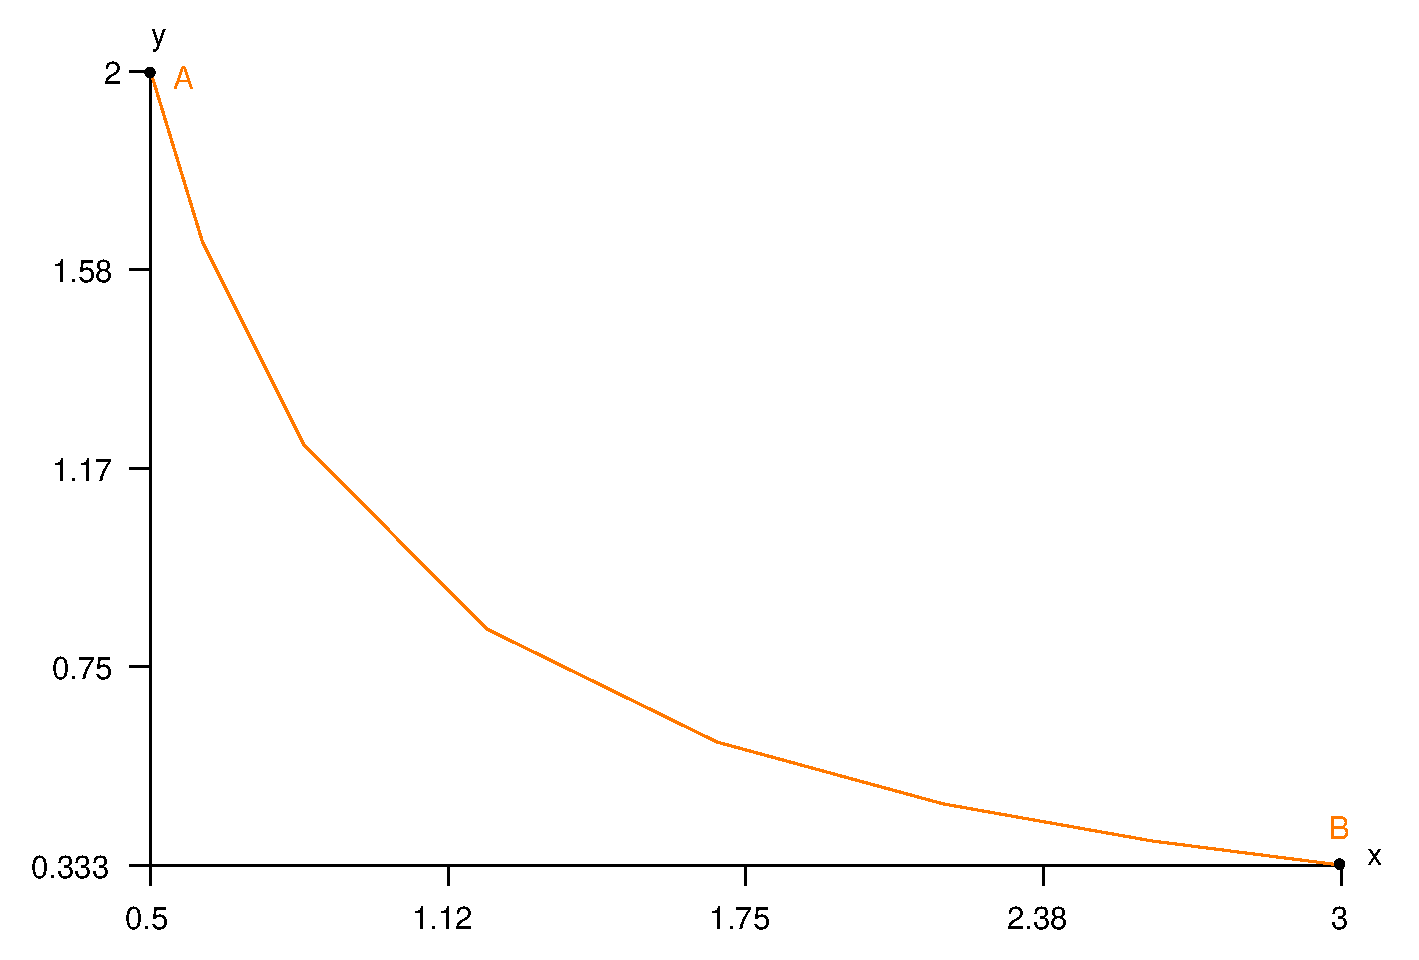
\includegraphics[width=75mm]{hiperbola.eps}} }

In {\tt gmsh}, you must select {\codett Tools} $\to$ {\codett Options} $\to$
{\codett Mesh} $\to$ {\codett 1D Elements} in order to see this mesh.

Note that the vertices are not perfectly uniformly distributed along the curve
because they are obtained as projections of points uniformly distributed along
the straight segment {\codett AB} onto the {\codett hiperbola} manifold.

Note also that when defining individual points {\codett A} and {\codett B} we must be careful
to set coordinates {\codett x} and {\codett y} within the {\codett hiperbola} manifold.
As an alternative, we might explicitly project them onto the {\codett hiperbola} like this :

\verbatim
   Cell P ( tag::vertex );  x(P) = 0.6;   y(P) = 2.1;
   hiperbola.project(P);
\endverbatim

\noindent In contrast, the {\codett Mesh} constructor with {\codett tag::segment} builds points
in the {\codett RR2} space and then projects them onto the {\codett hiperbola}
without the user's assistance.

The projection is done by applying a few steps of Newton's method for under-determined
(systems of) equations.%
\footnote *{\parbox{\ftntfont\baselineskip=3pt
See e.g.\ Appendix B in C.~Barbarosie, A.M.~Toader, S.~Lopes, A gradient-type algorithm for constrained
optimization with application to microstructure optimization, Discrete and Continuous Dynamical
Systems series B, 25, p.\ 1729-1755, 2020}}
Thus, it only works as expected for a point not too far from the manifold.

Paragraph \numb section 3.\numb parag 5 shows another way of meshing a curve,
producing equidistant vertices.


\paragraph{\numb section 2.\numb parag 4. A circle defined by four curved segments}

We can define several arcs of curve and {\codett join} them, thus obtaining a closed curve :
\medskip

\verbatim
   Manifold circle_manifold = RR2.implicit ( x*x + y*y == 1. );
   Cell N ( tag::vertex );  x(N) =  0.;   y(N) =  1.;
   Cell W ( tag::vertex );  x(W) = -1.;   y(W) =  0.;
   Cell S ( tag::vertex );  x(S) =  0.;   y(S) = -1.;
   Cell E ( tag::vertex );  x(E) =  1.;   y(E) =  0.;
   Mesh NW ( tag::segment, N.reverse(), W, tag::divided_in, 5 );
   Mesh WS ( tag::segment, W.reverse(), S, tag::divided_in, 5 );
   Mesh SE ( tag::segment, S.reverse(), E, tag::divided_in, 5 );
   Mesh EN ( tag::segment, E, N.reverse(), tag::divided_in, 5 );
   Mesh circle ( tag::join, NW, WS, SE, EN );
\endverbatim

{ \psfrag{N}{\special{ps: gsave 0 0 0.8 setrgbcolor}{\codett N}\special{ps: grestore}}
\psfrag{S}{\special{ps: gsave 0 0 0.8 setrgbcolor}{\codett S}\special{ps: grestore}}
\psfrag{E}{\special{ps: gsave 0 0 0.8 setrgbcolor}{\codett E}\special{ps: grestore}}
\psfrag{W}{\special{ps: gsave 0 0 0.8 setrgbcolor}{\codett W}\special{ps: grestore}}
\centerline{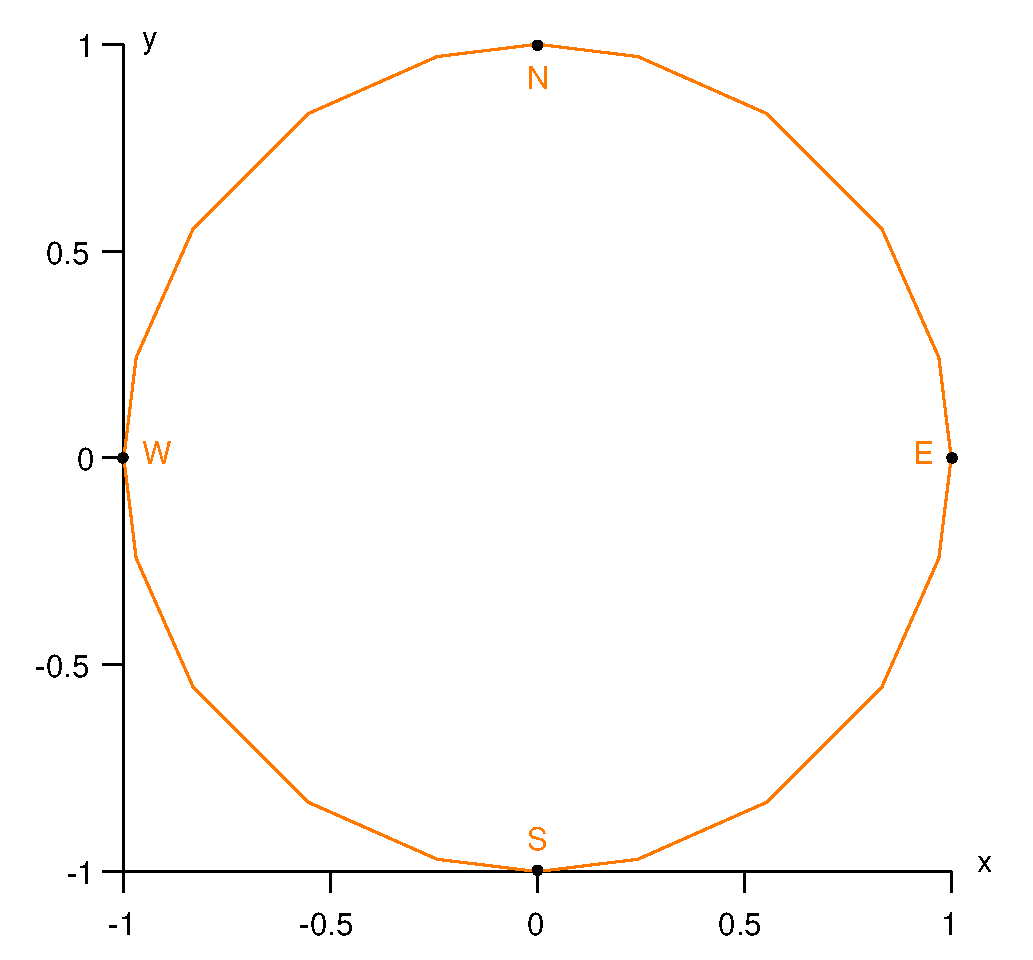
\includegraphics[width=70mm]{circle.eps}} }

Again, the vertices are not perfectly uniformly distributed along the circle
because they are obtained as projections (on the circle) of points along straight segments
{\codett NW}, {\codett WS} and so forth.

Note that applying the {\codett Mesh} constructor with {\codett tag::join} to four segments
is very different from applying the {\codett Mesh} constructor with {\codett tag::quadrangle}
to the same four segments; see paragraph \numb section 2.\numb parag 8.

Paragraph \numb section 3.\numb parag 2 shows another way of meshing a closed curve,
producing equidistant vertices.


\paragraph{\numb section 2.\numb parag 5. A hemisphere defined by four curved triangles}

Let's look at a surface in $ \RR^3 $ :

\verbatim
   Manifold RR3 ( tag::Euclid, tag::of_dim, 3 );
   Function xyz = RR3.build_coordinate_system ( tag::Lagrange, tag::of_degree, 1 );
   Function x = xyz[0],  y = xyz[1],  z = xyz[2];

   Manifold sphere = RR3.implicit ( x*x + y*y + z*z == 1. );

   // let's mesh half of a sphere
   Cell E  ( tag::vertex );   x(E) =  1.;   y(E) =  0.;   z(E) = 0.;
   Cell N  ( tag::vertex );   x(N) =  0.;   y(N) =  1.;   z(N) = 0.;
   Cell W  ( tag::vertex );   x(W) = -1.;   y(W) =  0.;   z(W) = 0.;
   Cell S  ( tag::vertex );   x(W) =  0.;   y(W) = -1.;   z(W) = 0.;
   Cell up ( tag::vertex );   x(up)=  0.;   y(up)=  0.;   z(up)= 1.;
   int n = 15;
   Mesh EN ( tag::segment, E.reverse(), N, tag::divided_in, n );
   Mesh NW ( tag::segment, N.reverse(), W, tag::divided_in, n );
   Mesh WS ( tag::segment, W.reverse(), S, tag::divided_in, n );
   Mesh SE ( tag::segment, S.reverse(), E, tag::divided_in, n );
   Mesh upE ( tag::segment, up.reverse(), E, tag::divided_in, n );
   Mesh upN ( tag::segment, up.reverse(), N, tag::divided_in, n );
   Mesh upW ( tag::segment, up.reverse(), W, tag::divided_in, n );
   Mesh upS ( tag::segment, up.reverse(), S, tag::divided_in, n );

   // build four triangles
   Mesh ENup ( tag::triangle, EN, upN.reverse(), upE );
   Mesh NWup ( tag::triangle, NW, upW.reverse(), upN );
   Mesh WSup ( tag::triangle, WS, upS.reverse(), upW );
   Mesh SEup ( tag::triangle, SE, upE.reverse(), upS );

   // and finally join the triangles :
   Mesh hemisphere ( tag::join, ENup, NWup, WSup, SEup );
\endverbatim

{ \psfrag{W}{\special{ps: gsave 0 0 0.8 setrgbcolor}{\codett W}\special{ps: grestore}}
\psfrag{S}{\special{ps: gsave 0 0 0.8 setrgbcolor}{\codett S}\special{ps: grestore}}
\psfrag{up}{\special{ps: gsave 0 0 0.8 setrgbcolor}{\codett up}\special{ps: grestore}}
\centerline{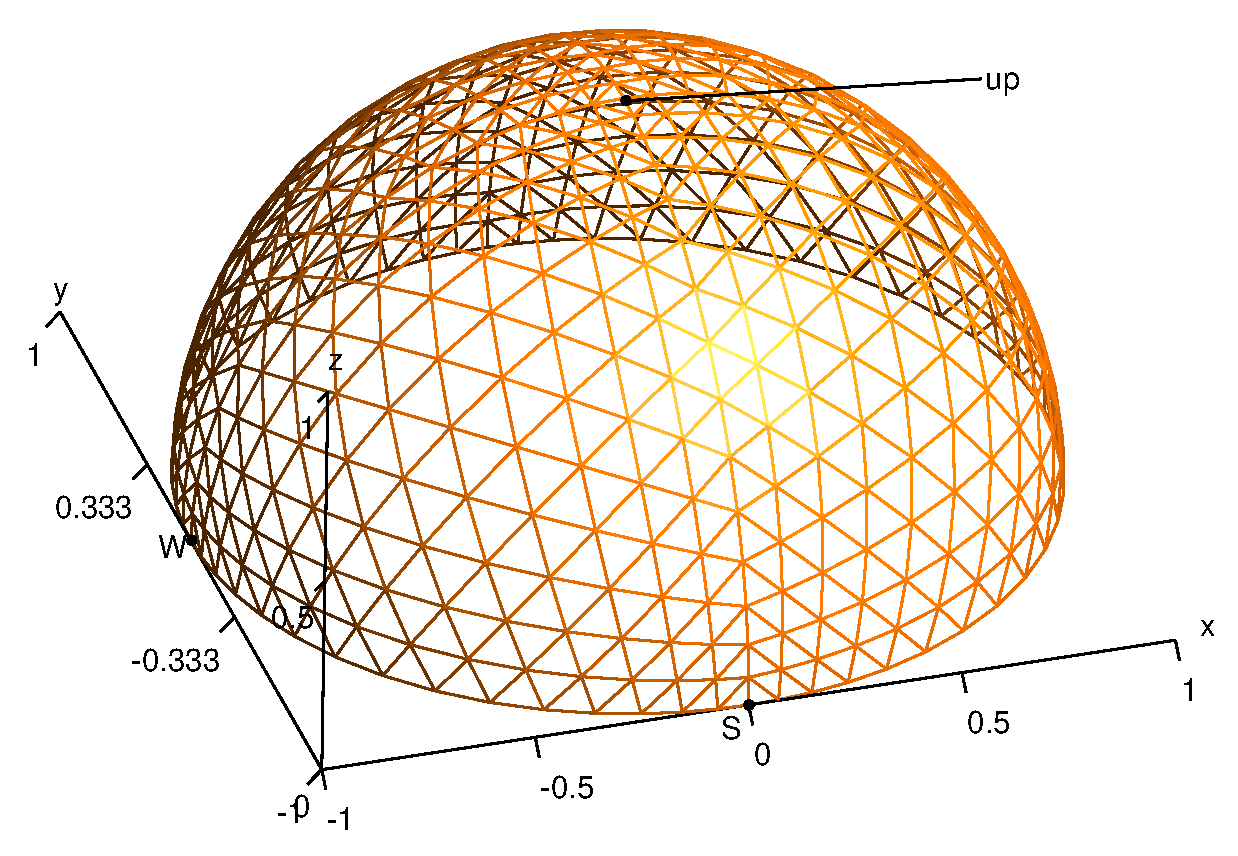
\includegraphics[width=10cm]{hemisphere.eps}} }

Again, when we define individual points {\codett E}, {\codett N}, {\codett W}, {\codett S} and
{\codett up} we must be careful to provide coordinates on the {\codett sphere}
(or {\codett project} them explicitly as shown in paragraph \numb section 2.\numb parag 6).
In contrast, the {\codett Mesh} constructors with {\codett tag::segment}, {\codett tag::quadrangle}
and {\codett tag::triangle} build points in the surrounding space ($ \RR^2 $ or $ \RR^3 $) and
then project them onto the current manifold without the user's assistance.
The projection is done by applying a few steps of Newton's method for under-determined
(systems of) equations.%
\footnote *{\parbox{\ftntfont\baselineskip=3pt
See e.g.\ Appendix B in C.~Barbarosie, A.M.~Toader, S.~Lopes, A gradient-type algorithm for constrained
optimization with application to microstructure optimization, Discrete and Continuous Dynamical
Systems series B, 25, p.\ 1729-1755, 2020}}
As a side effect, within each triangle ({\codett ENup}, {\codett NWup} and so forth),
the distribution of the vertices is not perfectly uniform.

Note that, when we build the segments {\codett WS}, {\codett upS} and so on,
we know that those segments will be (polygonal approximatins of) arcs of circle on the sphere.
This is so due to the particular geometry of our manifold (we know that the projection of
a straight line segment on the sphere is an arc of circle of radius equal to the radius of
the sphere); the shape of such segments is less clear in other examples
(like the one in paragraph \numb section 2.\numb parag 6).

Section \numb section 3 shows other ways of meshing a surface.


\paragraph{\numb section 2.\numb parag 6. A more complex surface}

If the surface is more ``bumpy'',
% since the projection operation doesn't work well for points far from the manifold,
we must use smaller patches in order to get a mesh of good quality.

Below we use twelve rectangles to get a bumpy hemisphere.

\verbatim
   Manifold nut = RR3.implicit ( x*x + y*y + z*z + 1.5*x*y*z == 1. );

   // let's mesh a hemisphere (much deformed)
   Cell S ( tag::vertex );    x(S)  =   0.;   y(S)  =  -1.;   z(S)  =  0.;
   Cell E ( tag::vertex );    x(E)  =   1.;   y(E)  =   0.;   z(E)  =  0.;
   Cell N ( tag::vertex );    x(N)  =   0.;   y(N)  =   1.;   z(N)  =  0.;
   Cell W ( tag::vertex );    x(W)  =  -1.;   y(W)  =   0.;   z(W)  =  0.;
   Cell up ( tag::vertex );   x(up) =   0.;   y(up) =   0.;   z(up) =  1.;
   // no need to project these
   Cell mSW ( tag::vertex );  x(mSW) = -1.;   y(mSW) = -1.;   z(mSW) = 0.;
   nut.project ( mSW );  // midway between S and W
   Cell mSup  ( tag::vertex );  x(mSup) =  0.;   y(mSup) = -1.;   z(mSup) = 1.;
   nut.project ( mSup );  // midway between S and up
   Cell mSWup ( tag::vertex );  x(mSWup) = -1.;  y(mSWup) = -1.;  z(mSWup) = 1.;
   nut.project ( mSWup );  // somewhere between S, W and up
   // ... and so forth ...
\endverbatim
	
{ \psfrag{W}{\special{ps: gsave 0 0 0.8 setrgbcolor}{\codett W}\special{ps: grestore}}
\psfrag{S}{\special{ps: gsave 0 0 0.8 setrgbcolor}{\codett S}\special{ps: grestore}}
\psfrag{mWS}{\special{ps: gsave 0 0 0.8 setrgbcolor}{\codett mSW}\special{ps: grestore}}
\psfrag{mSE}{\special{ps: gsave 0 0 0.8 setrgbcolor}{\codett mSE}\special{ps: grestore}}
\psfrag{mWup}{\special{ps: gsave 0 0 0.8 setrgbcolor}{\codett mWup}\special{ps: grestore}}
\psfrag{mSup}{\special{ps: gsave 0 0 0.8 setrgbcolor}{\codett mSup}\special{ps: grestore}}
\psfrag{mSEup}{\special{ps: gsave 0 0 0.8 setrgbcolor}{\codett mSEup}\special{ps: grestore}}
\psfrag{up}{\special{ps: gsave 0 0 0.8 setrgbcolor}{\codett up}\special{ps: grestore}}
\psfrag{mWSup}{\special{ps: gsave 0 0 0.8 setrgbcolor}{\codett mSWup}\special{ps: grestore}}
\centerline{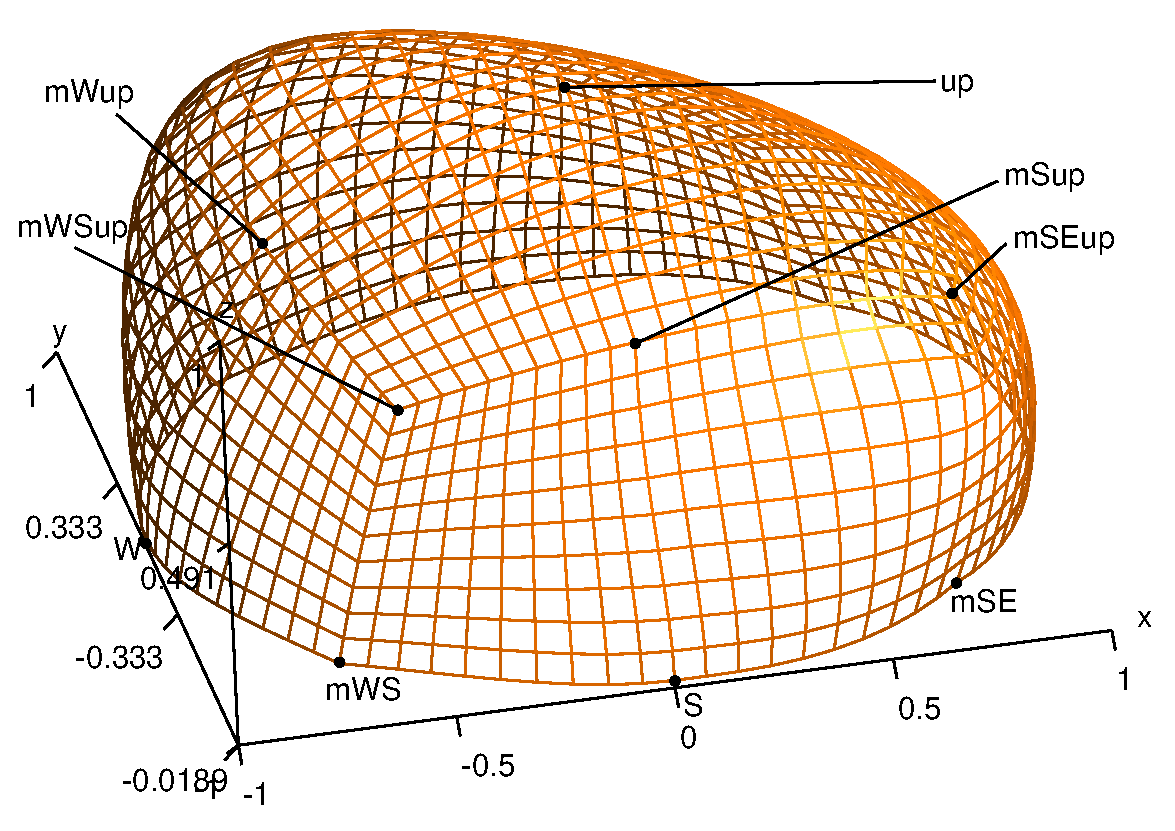
\includegraphics[width=10cm]{hemisphere-2.eps}} }

\verbatim
   // now build segments :
   int n = 10;
   Mesh W_mSW  ( tag::segment, W.reverse(), mSW,  tag::divided_in, n );
   Mesh W_mWup ( tag::segment, W.reverse(), mWup, tag::divided_in, n );
   // ... and so forth ...

   // now the twelve rectangles :
   Mesh rect_W_SW  ( tag::quadrangle,
      mSW_mSWup, mWup_mSWup.reverse(), W_mWup.reverse(), W_mSW );
   Mesh rect_S_SW  ( tag::quadrangle,
      mSup_mSWup, mSW_mSWup.reverse(), S_mSW.reverse(), S_mSup );
   Mesh rect_up_SW ( tag::quadrangle,
      mWup_mSWup, mSup_mSWup.reverse(), up_mSup.reverse(), up_mWup );
   // ... and so forth ...

   // and finally join the rectangles :
   Mesh hemisphere ( tag::join,
      { rect_E_NE, rect_E_SE, rect_S_SE, rect_S_SW, rect_W_SW, rect_W_NW,
        rect_N_NE, rect_N_NW, rect_up_SE, rect_up_SW, rect_up_NE, rect_up_NW } );
\endverbatim

Note how we use a version of the {\codett Mesh} constructor with {\codett tag::join} taking as
argument a list of {\codett Mesh}es; the same constructor is used in paragraph \numb section
8.\numb parag 2.

Unlike in paragraph \numb section 2.\numb parag 5, here we do not control the
exact shape of the segments {\codett S\_mSW}, {\codett S\_mSup} and so on.
They are projections of straight line segments onto our surface but since the equation
of the surface is rather complicated we do not know the exact shape of these projections.
Since points like {\codett mSW} and {\codett mSE} have been placed initially in {\codett RR3}
not belonging to the {\codett bupmy} manifold and then explicitly {\codett project}ed,
there is no guarantee that they lie in the plane $ z = 0 $ (they probably don't).
We notice an angle between {\codett W\_mSW} and {\codett S\_mSW} at {\codett mSW}.

Paragraph \numb section 2.\numb parag 12 shows a way to control the shape of the segments
{\codett S\_mSW}, {\codett S\_mSE} and so on.

Section \numb section 3 shows other ways of meshing a surface.


\paragraph{\numb section 2.\numb parag 7. Exercise}

Slightly change the code in paragraph \numb section 2.\numb parag 6
in order to obtain the mesh below.
(Hint: have a look at paragraph \numb section 2.\numb parag 2.)

\centerline{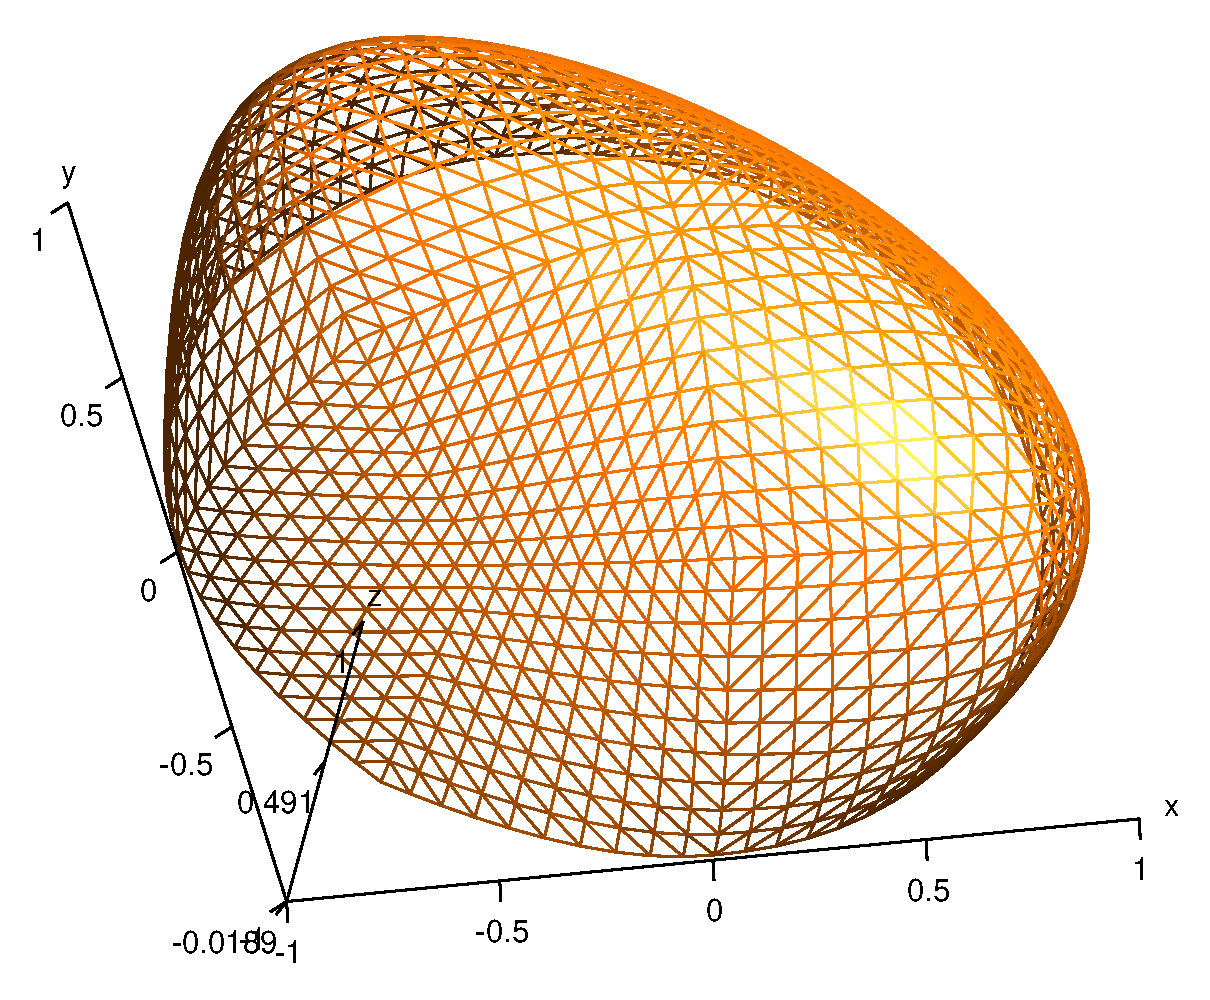
\includegraphics[width=99mm]{hemisphere-1.eps}}
\vfil\eject


\paragraph{\numb section 2.\numb parag 8. Alternating between manifolds}

Let's go back to the example in paragraph \numb section 2.\numb parag 4.
Suppose we want to mesh the whole disk, not just its boundary.
We can build the boundary of the disk just like in paragraph \numb section 2.\numb parag 4,
by placing ourselves in the manifold {\codett circle}.
But if we want to mesh the interior of the disk, we must leave {\codett circle} and
switch back to the original {\codett RR2} manifold.
Method {\codett set\_as\_working\_manifold} allows us to do that.

\verbatim
   Manifold RR2 ( tag::Euclid, tag::of_dim, 2 );
   Function xy = RR2.build_coordinate_system ( tag::Lagrange, tag::of_degree, 1 );
   Function x = xy[0],  y = xy[1];
   
   Manifold circle = RR2.implicit ( x*x + y*y == 1. );
   
   Cell N ( tag::vertex );  x(N) =  0.;   y(N) =  1.;
   Cell W ( tag::vertex );  x(W) = -1.;   y(W) =  0.;
   Cell S ( tag::vertex );  x(S) =  0.;   y(S) = -1.;
   Cell E ( tag::vertex );  x(E) =  1.;   y(E) =  0.;
   Mesh NW ( tag::segment, N.reverse(), W, tag::divided_in, 10 );
   Mesh WS ( tag::segment, W.reverse(), S, tag::divided_in, 10 );
   Mesh SE ( tag::segment, S.reverse(), E, tag::divided_in, 10 );
   Mesh EN ( tag::segment, E.reverse(), N, tag::divided_in, 10 );
   
   RR2.set_as_working_manifold();
   Mesh disk ( tag::quadrangle, NW, WS, SE, EN );
\endverbatim

{ \psfrag{N}{\special{ps: gsave 0 0 0.8 setrgbcolor}{\codett N}\special{ps: grestore}}
\psfrag{S}{\special{ps: gsave 0 0 0.8 setrgbcolor}{\codett S}\special{ps: grestore}}
\psfrag{E}{\special{ps: gsave 0 0 0.8 setrgbcolor}{\codett E}\special{ps: grestore}}
\psfrag{W}{\special{ps: gsave 0 0 0.8 setrgbcolor}{\codett W}\special{ps: grestore}}
\centerline{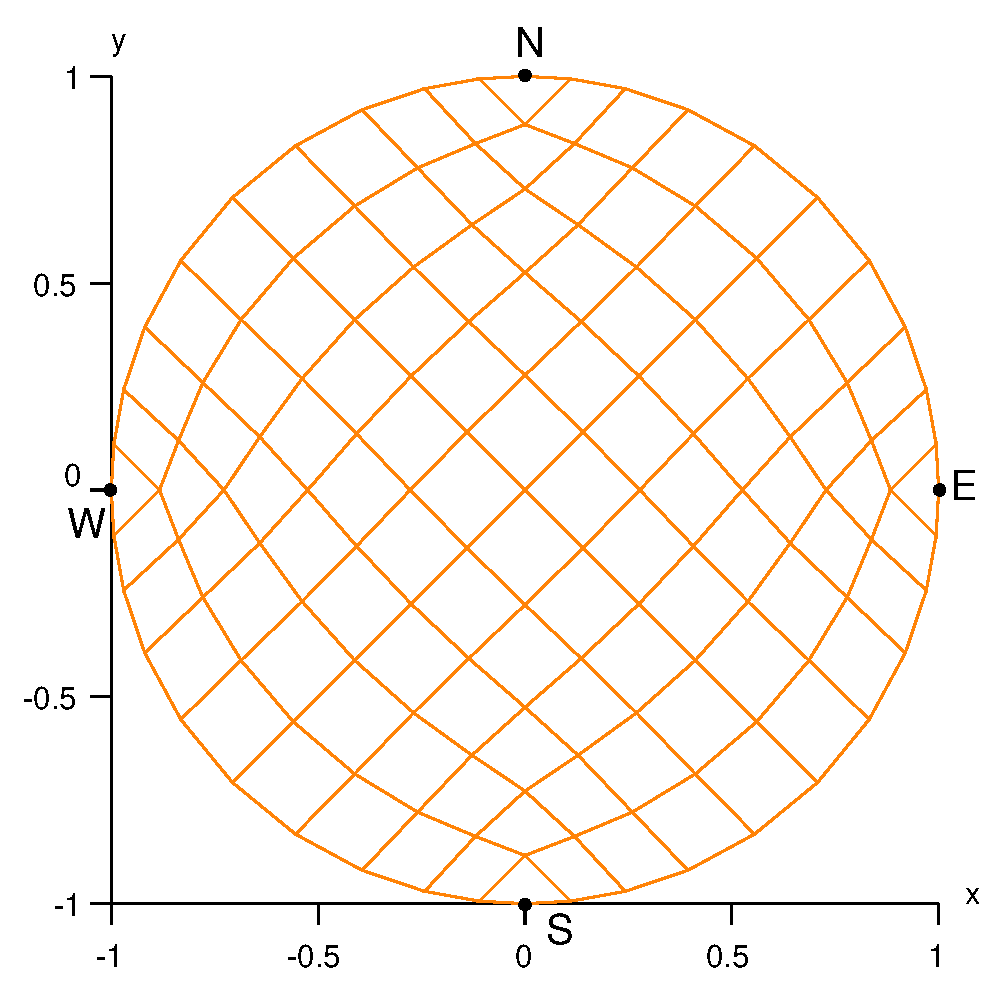
\includegraphics[width=70mm]{disk.eps}} }

The mesh is of poor quality; we obtain quadrilaterals having a wide angle near {\codett S},
{\codett N}, {\codett E} and {\codett W}.
Paragraphs \numb section 3.\numb parag 1 and \numb section 3.\numb parag 2 show another way
of meshing a disk, having its boundary as starting point.

Each time a {\codett Manifold} object is created, its constructor sets it as working manifold;
this is why in many cases we don't need to know about method {\codett set\_as\_working\_manifold}.
We need it, however, in cases like the one presented here.
\vfil\eject


\paragraph{\numb section 2.\numb parag 9. Alternating between manifolds, again}

Here is an example similar to the one in paragraph \numb section 2.\numb parag 8,
this time with four arcs of hiperbola.

\verbatim
   Manifold RR2 ( tag::Euclid, tag::of_dim, 2 );
   Function xy = RR2.build_coordinate_system ( tag::Lagrange, tag::of_degree, 1 );
   Function x = xy[0],  y = xy[1];

   Cell N ( tag::vertex );  x(N) =  0.;   y(N) =  1.;
   Cell W ( tag::vertex );  x(W) = -1.;   y(W) =  0.;
   Cell S ( tag::vertex );  x(S) =  0.;   y(S) = -1.;
   Cell E ( tag::vertex );  x(E) =  1.;   y(E) =  0.;

   Manifold first_arc  = RR2.implicit ( x*y + x - y == -1. );
   Mesh NW ( tag::segment, N.reverse(), W, tag::divided_in, 10 );
   Manifold second_arc = RR2.implicit ( x*y - x - y ==  1. );
   Mesh WS ( tag::segment, W.reverse(), S, tag::divided_in, 10 );
   Manifold third_arc  = RR2.implicit ( x*y - x + y == -1. );
   Mesh SE ( tag::segment, S.reverse(), E, tag::divided_in, 10 );
   Manifold fourth_arc = RR2.implicit ( x*y + x + y ==  1. );
   Mesh EN ( tag::segment, E.reverse(), N, tag::divided_in, 10 );
   
   RR2.set_as_working_manifold();
   Mesh diamond ( tag::quadrangle, NW, WS, SE, EN );
\endverbatim

{ \psfrag{N}{\special{ps: gsave 0 0 0.8 setrgbcolor}{\codett N}\special{ps: grestore}}
\psfrag{S}{\special{ps: gsave 0 0 0.8 setrgbcolor}{\codett S}\special{ps: grestore}}
\psfrag{E}{\special{ps: gsave 0 0 0.8 setrgbcolor}{\codett E}\special{ps: grestore}}
\psfrag{W}{\special{ps: gsave 0 0 0.8 setrgbcolor}{\codett W}\special{ps: grestore}}
\centerline{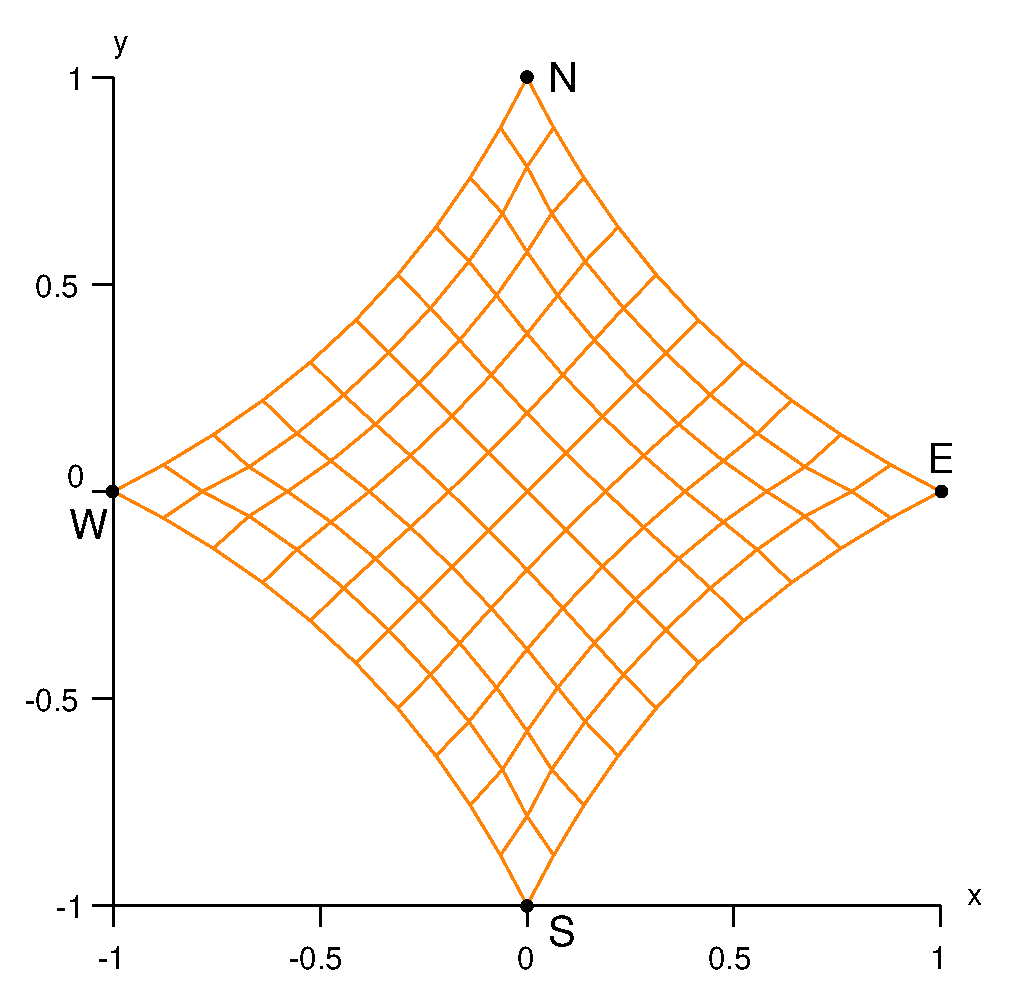
\includegraphics[width=75mm]{diamond.eps}} }

Paragraph \numb section 3.\numb parag 17 shows another way of meshing the same domain.
\vfil\eject


\paragraph{\numb section 2.\numb parag 10. An organic shape}

This paragraph describes a surface meant to mimik the shape of a physalis fruit.

$$ 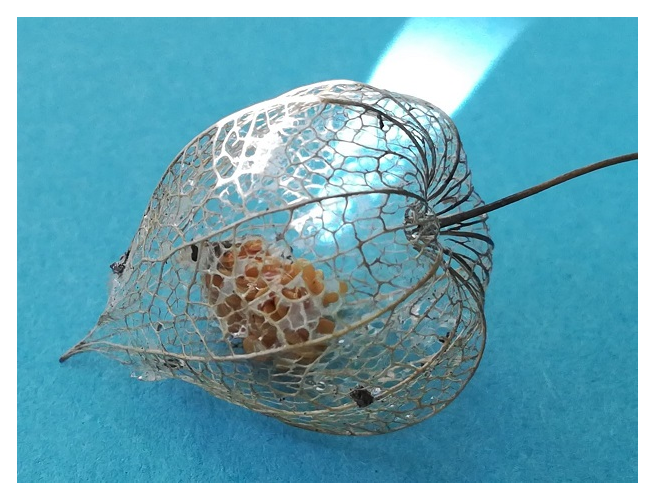
\includegraphics[width=85mm]{dry-physalis.eps} $$
\vskip 2mm

We begin by defining a revolution surface in $ \RR^3 $ :

\verbatim
   Function r2 = x*x + y*y + z*z;
   const double pi = 3.1415926536;
   Manifold apple = RR3.implicit ( power(r2,0.5) * sin(r2-pi/6.) == z );
\endverbatim

This surface has the shape shown below, which does not resemble a physalis fruit.

$$ 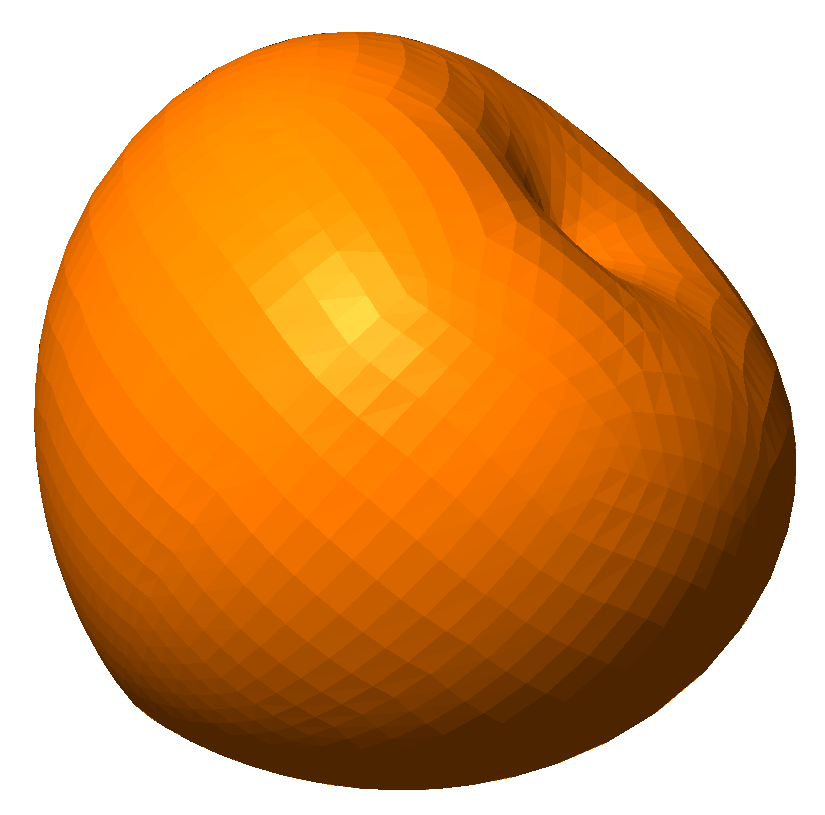
\includegraphics[width=80mm]{fisalis-manif.eps} $$

\vfil\eject
Instead of meshing the {\codett apple} surface, we just build eight curves immersed in it
(each curve joins {\codett A} to {\codett D} and is made of three segments) :

\verbatim
   Cell A ( tag::vertex );  x(A) =  0.;  y(A) =  0.;  z(A) = std::sqrt ( 2.*pi/3. );
   Cell B1 ( tag::vertex );  x(B1) =  1.;  y(B1) =  0.;  z(B1) =  1.;
   Cell C1 ( tag::vertex );  x(C1) =  1.;  y(C1) =  0.;  z(C1) =  0.;
   apple.project (B1);  apple.project (C1);
   Cell D ( tag::vertex );  x(D) =  0.;  y(D) =  0.;  z(D) =  0.;
   Mesh AB1 ( tag::segment, A.reverse(), B1, tag::divided_in, 10 );
   Mesh B1C1 ( tag::segment, B1.reverse(), C1, tag::divided_in, 10 );
   Mesh C1D ( tag::segment, C1.reverse(), D, tag::divided_in, 10 );
   // and so on ...
\endverbatim

Then we switch back to {\codett RR3} (thus leaving the {\codett apple} manifold) and build
transversal segments, as well as triangular and quadrangular patches :

\verbatim
   RR3.set_as_working_manifold();
   Mesh B1B2 ( tag::segment, B1.reverse(), B2, tag::divided_in, 10 );
   Mesh B2B3 ( tag::segment, B2.reverse(), B3, tag::divided_in, 10 );
   // and many other segments ...
   Mesh AB1B2 ( tag::triangle, AB1, B1B2, AB2.reverse() );
   Mesh AB2B3 ( tag::triangle, AB2, B2B3, AB3.reverse() );
   // and other triangular patches ...
   Mesh B1C1C2B2 ( tag::quadrangle, B1C1, C1C2, B2C2.reverse(), B1B2.reverse(),
                   tag::with_triangles                                           );
   Mesh B2C2C3B3 ( tag::quadrangle, B2C2, C2C3, B3C3.reverse(), B2B3.reverse(),
                   tag::with_triangles                                           );
   // and other quadrangular patches ...   
\endverbatim

We then join all patches :
\verbatim
   Mesh sect1 ( tag::join, AB1B2, B1C1C2B2, C1DC2 );
   Mesh sect2 ( tag::join, AB2B3, B2C2C3B3, C2DC3 );
   // more sectors ...
   std::list < Mesh > lm { sect1, sect2, sect3, sect4, sect5, sect6, sect7, sect8 };
   Mesh fisalis ( tag::join, lm ); 
\endverbatim

$$ 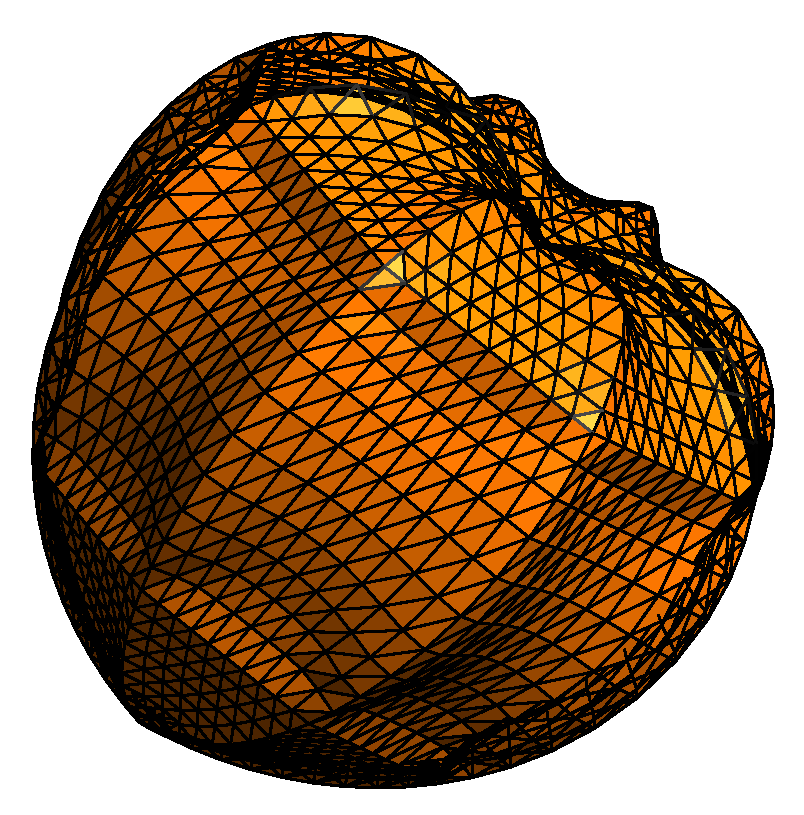
\includegraphics[width=60mm]{fisalis-round.eps} $$

This shape is still not satisfactory, so we apply a deformation in $ \RR^3 $ in order to
get a sharper tip.
The {\codett apple} manifold is no longer relevant.

\verbatim
   CellIterator it = fisalis.iter_over ( tag::vertices );
   for ( it.reset(); it.in_range(); it++ )
   {  Cell P = *it;
      x(P) *= 0.8;  y(P) *= 0.8;
      if ( z(P) > 1.3 )
      {	 x(P) = x(P) / ( 1. + 300. * std::pow ( z(P) - 1.3, 3. ) );
         y(P) = y(P) / ( 1. + 300. * std::pow ( z(P) - 1.3, 3. ) );
         z(P) = z(P) * ( 1. + 10. * ( z(P) - 1.3 ) * ( z(P) - 1.3 ) );  }
      if ( z(P) > 0. ) z(P) *= 0.8;                                        }
\endverbatim

We add a sequence of baricenter operations for smoothening the shape.
Note that each baricenter operation is relative to a sector and it applies only to inner
vertices, so the boundary of the sector is not changed.
Thus, the eight rims defined in the beginning are kept unchanged.

\verbatim
   std::list<Mesh>::iterator it1;
   for ( it1 = lm.begin(); it1 != lm.end(); it1++ )
   {  Mesh sect = *it1;
      CellIterator it2 = sect.iter_over ( tag::cells_of_dim, 1 );
      for ( int i = 1; i < 20; i++ )
      for ( it2.reset(); it2.in_range(); it2++ )
      {  Cell seg = *it2;
         sect.baricenter ( seg.tip(), seg );
         seg = seg.reverse();
         sect.baricenter ( seg.tip(), seg );  }                     }
\endverbatim

And we are happy with the final result :

$$ 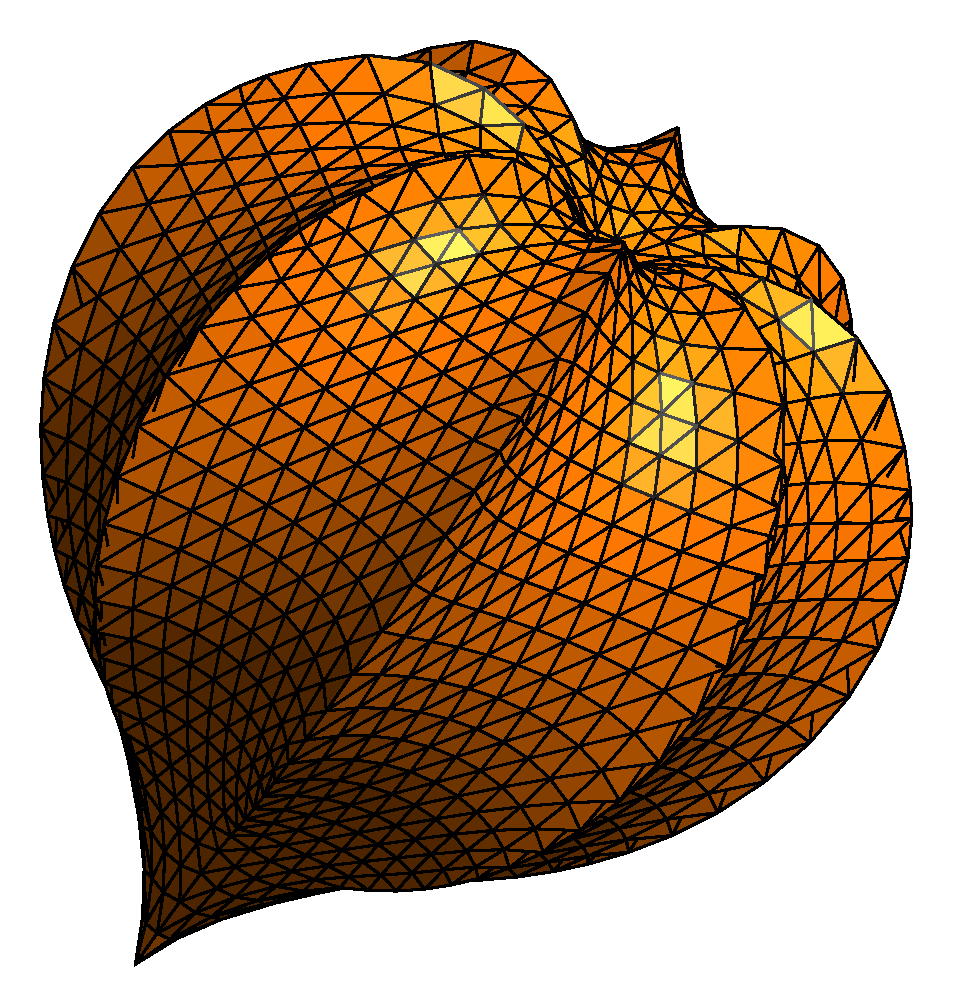
\includegraphics[width=75mm]{fisalis.eps} $$


\paragraph{\numb section 2.\numb parag 11. A manifold defined by two equations}

We can define a one-dimensional submanifold of $ \RR^3 $ by two implicit equations :
\medskip

\verbatim
   Manifold RR3 ( tag::Euclid, tag::of_dim, 3 );
   Function xyz = RR3.build_coordinate_system ( tag::Lagrange, tag::of_degree, 1 );
   Function x = xyz[0],  y = xyz[1],  z = xyz[2];

   Manifold circle_manifold = RR3.implicit ( x*x + y*y == 1., x*y == 4.*z );
   Cell S ( tag::vertex );  x(S) =  0.;   y(S) = -1.;  z(S) = 0.;
   Cell E ( tag::vertex );  x(E) =  1.;   y(E) =  0.;  z(E) = 0.;
   Cell N ( tag::vertex );  x(N) =  0.;   y(N) =  1.;  z(N) = 0.;
   Cell W ( tag::vertex );  x(W) = -1.;   y(W) =  0.;  z(W) = 0.;
   // these four points already belong to 'circle_manifold', no projection needed
   Mesh SE ( tag::segment, S.reverse(), E, tag::divided_in, 5 );
   Mesh EN ( tag::segment, E.reverse(), N, tag::divided_in, 5 );
   Mesh NW ( tag::segment, N.reverse(), W, tag::divided_in, 5 );
   Mesh WS ( tag::segment, W.reverse(), S, tag::divided_in, 5 );
   Mesh circle ( tag::join, SE, EN, NW, WS );
\endverbatim

{ \psfrag{N}{\special{ps: gsave 0 0 0.8 setrgbcolor}{\codett N}\special{ps: grestore}}
\psfrag{S}{\special{ps: gsave 0 0 0.8 setrgbcolor}{\codett S}\special{ps: grestore}}
\psfrag{E}{\special{ps: gsave 0 0 0.8 setrgbcolor}{\codett E}\special{ps: grestore}}
\psfrag{W}{\special{ps: gsave 0 0 0.8 setrgbcolor}{\codett W}\special{ps: grestore}}
\centerline{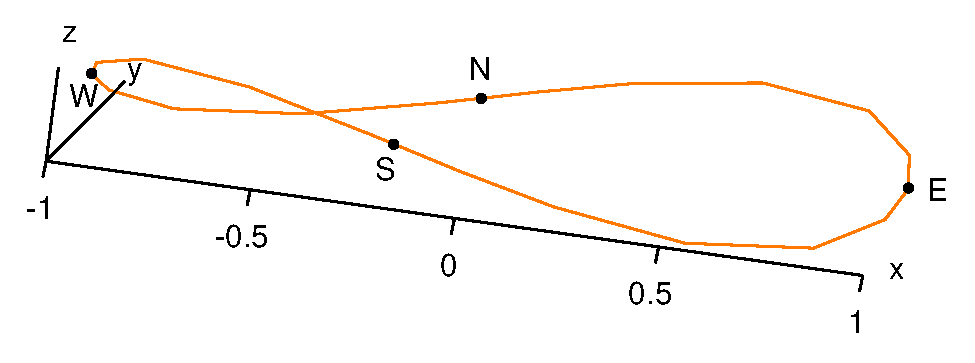
\includegraphics[width=85mm]{circle-3d.eps}} }

Paragraph \numb section 3.\numb parag 4 shows another way of meshing the same loop.


\paragraph{\numb section 2.\numb parag 12. A submanifold of a submanifold}

An implicit manifold has submanifolds.
For instance, we can improve the look of the ``bumpy hemisphere'' in paragraph
\numb section 2.\numb parag 6 by building its base (a circle-like closed curve)
inside a one-dimensional manifold.
For the rest of the surface, we switch back to the two-dimensional manifold {\codett nut} :
\medskip

\verbatim
   Manifold nut = RR3.implicit ( x*x + y*y + z*z + 1.5*x*y*z == 1. );
   int n = 10;

   // first build the base (a closed curve) 
   Manifold base = nut.implicit ( x*x + 3.*z == 0. );

   Cell S ( tag::vertex );    x(S)  =   0.;   y(S)  =  -1.;   z(S)  =  0.;
   Cell E ( tag::vertex );    x(E)  =   1.;   y(E)  =   0.;   z(E)  =  0.;
   Cell N ( tag::vertex );    x(N)  =   0.;   y(N)  =   1.;   z(N)  =  0.;
   Cell W ( tag::vertex );    x(W)  =  -1.;   y(W)  =   0.;   z(W)  =  0.;
   // no need to project S and N, they are already on 'base'
   base.project(E);  base.project(W);
   Cell mSW ( tag::vertex );  x(mSW) = -1.;   y(mSW) = -1.;   z(mSW) = 0.;
   base.project ( mSW );  // midway between S and W
   Cell mSE ( tag::vertex );  x(mSE) =  1.;   y(mSE) = -1.;   z(mSW) = 0.;
   base.project ( mSE );  // midway between S and E
   // define similarly mNE and mNW

   // now build eight segments, forming the base
   Mesh W_mSW  ( tag::segment, W.reverse(), mSW, tag::divided_in, n );
   Mesh S_mSW  ( tag::segment, S.reverse(), mSW, tag::divided_in, n );
   // define similarly S_mSE, E_mSE, E_mNE, N_mNE, N_mNW, W_mNW

   // we are done with the base, now switch back to 'nut'
   nut.set_as_working_manifold();

   // more points :
   Cell up ( tag::vertex );   x(up) =   0.;   y(up) =   0.;   z(up) =  1.;
   // no need to project 'up', it is already on 'nut'
   Cell mSup  ( tag::vertex );  x(mSup) =  0.;   y(mSup) = -1.;   z(mSup) = 1.;
   nut.project ( mSup );  // midway between S and up
   Cell mSWup ( tag::vertex );  x(mSWup) = -1.;  y(mSWup) = -1.;  z(mSWup) = 1.;
   nut.project ( mSWup );  // somewhere between S, W and up
   // ... and so forth ...

   // more segments :
   Mesh W_mWup ( tag::segment, W.reverse(), mWup, tag::divided_in, n );
   Mesh mSW_mSWup ( tag::segment, mSW.reverse(), mSWup, tag::divided_in, n );
   Mesh mWup_mSWup ( tag::segment, mWup.reverse(), mSWup, tag::divided_in, n );
   // ... and so forth ...
\endverbatim

\centerline{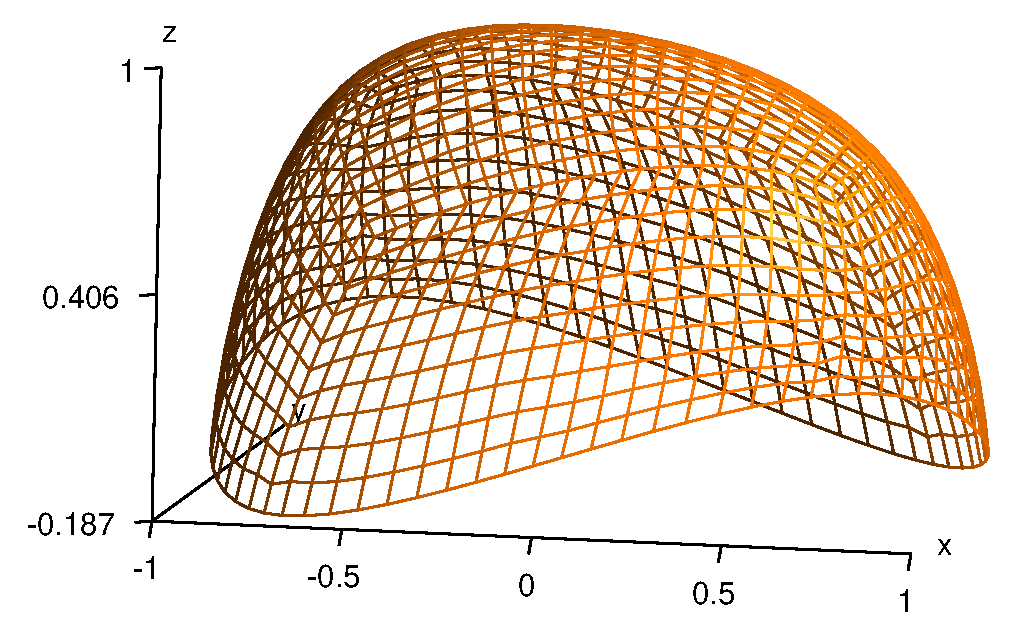
\includegraphics[width=9cm]{bumpy.eps}}

If we wanted a flat base, we could have defined

\verbatim
   Manifold base = nut.implicit ( z == 0. );
\endverbatim

Paragraph \numb section 3.\numb parag 9 shows a way to mesh the same surface using
fewer lines of code.


\paragraph{\numb section 2.\numb parag 13. Parametric manifolds -- a curve}

Paragraphs \numb section 2.\numb parag 3 -- \numb section 2.\numb parag 12 describe manifolds
defined through implicit equations, that is, level sets in $ \RR^2 $ or $ \RR^3 $.
Another way of defining a submanifold is through a parametrization.
Below is an example.

\verbatim
   // at the beginning, we define 'spiral' as a straight line
   Manifold spiral ( tag::Euclid, tag::of_dim, 1 );
   Function t = spiral.build_coordinate_system ( tag::Lagrange, tag::of_degree, 1 );

   // now build 'arc_of_spiral' merely as a segment from pi/2 to 5 pi
   const double pi = 3.1415926536;
   Cell A ( tag::vertex );  t(A) =  pi/2.;
   Cell B ( tag::vertex );  t(B) =  5.*pi;
   Mesh arc_of_spiral ( tag::segment, A.reverse(), B, tag::divided_in, 30 );

   // not very interesting for now
   // but now define functions x and y as expressions of t :
   Function x = t*cos(t), y = t*sin(t);

   // and declare them to be the new coordinates on the 'spiral' manifold
   spiral.set_coordinates ( x && y );

   // in future statements (e.g. for graphical representation)
   // x and y will be used, not t :
   arc_of_spiral.draw_ps ("spiral.eps");
\endverbatim

{ \psfrag{A}{\special{ps: gsave 0 0 0.8 setrgbcolor}{\codett A}\special{ps: grestore}}
\psfrag{B}{\special{ps: gsave 0 0 0.8 setrgbcolor}{\codett B}\special{ps: grestore}}
\centerline{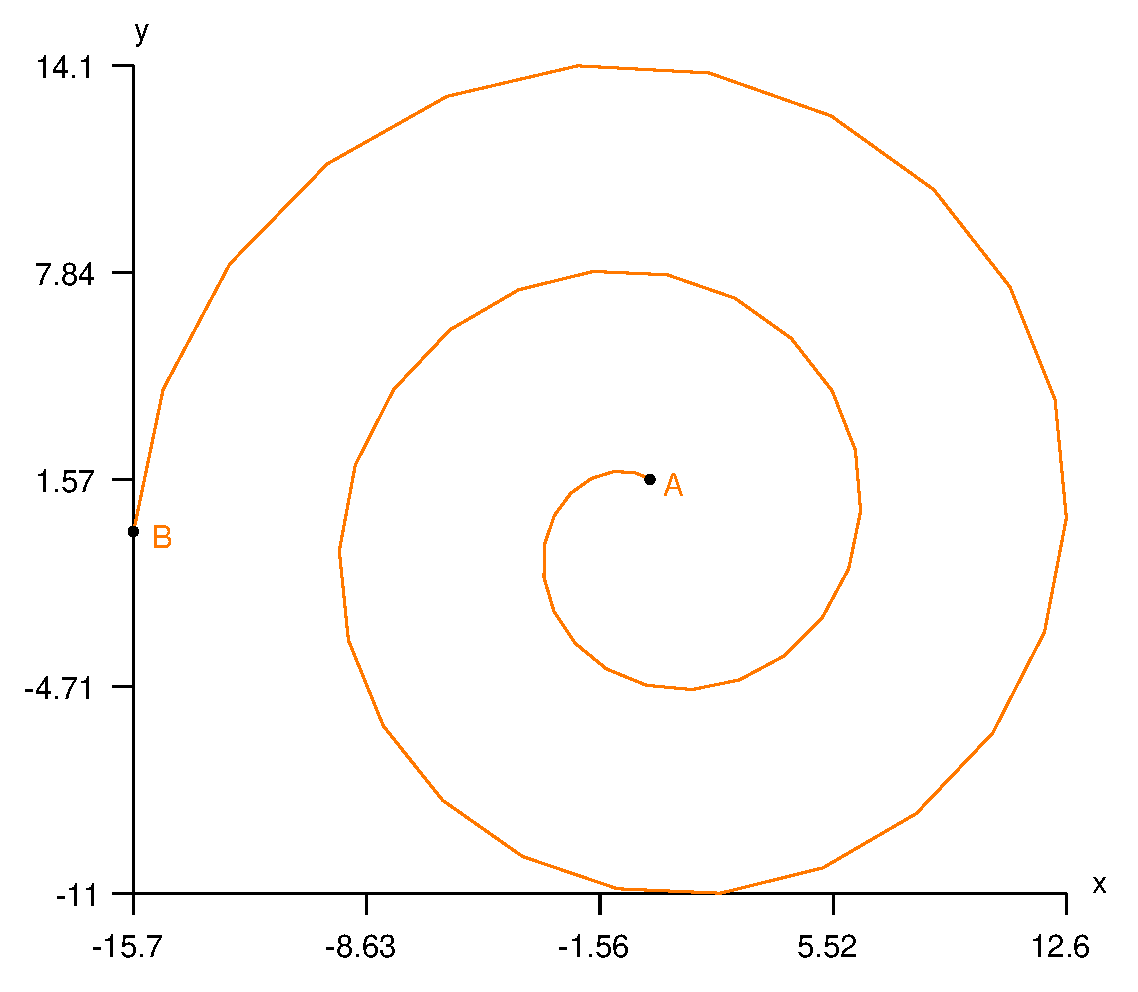
\includegraphics[width=65mm]{spiral.eps}} }

The operator {\codett \&\&} joins two functions into one vector function.

Note that, when defining points {\codett A} and {\codett B}, we only set the value of {\codett t}.
Functions {\codett x} and {\codett y} are defined later, as arithmetic expressions in terms of
{\codett t}; their values will be computed ``on-the-fly'' when needed.
%A parametric manifold has attached to it a function called ``parameter'' and another one called
%``coordinate''.
%Both may be vector functions (may have serveral components).
%The ``coordinates'' are used, for instance, for graphical representation.
%The ``parameter'' or ``parameters'' are used, for instance, for interpolation.
%The {\codett Mesh} constructors with {\codett tag::segment}, {\codett tag::quadrangle} or
%{\codett tag::triangle} build new points and define their position in the manifold by
%interpolating the parameters, not the coordinates.
%Unlike for implicit manifolds, no projection is necessary.
In the drawing above, we note that the generated points are not equidistant in the sense of the
Euclidian distance in $ \RR^2 $.
They correspond to values of {\codett t} which are uniformly distributed between
$ \pi/2 $ (at {\codett A}) and $ 5\pi $ (at {\codett B}).

The approach described above has the disadvantage that, if we want to subsequently change the
distribution of nodes along the {\codett arc\_of\_spiral}, we must switch back to the original
{\codett t} coordinate.

Paragraph \numb section 3.\numb parag 5 shows another way of meshing a curve,
producing equidistant vertices.


\paragraph{\numb section 2.\numb parag 14. Closing a circle}

In the approach of paragraph \numb section 2.\numb parag 13, it is possible but cumbersome to
build a closed curve :

\verbatim
   Manifold circle_manif ( tag::Euclid, tag::of_dim, 1 );
   Function t = circle_manif.build_coordinate_system
      ( tag::Lagrange, tag::of_degree, 1 );

   // build 'circle' merely as a segment from 0 to 1.9 pi
   const double pi = 3.1415926536;
   Cell A ( tag::vertex );  t(A) =  0.;
   Cell B ( tag::vertex );  t(B) =  1.9*pi;
   Mesh circle ( tag::segment, A.reverse(), B, tag::divided_in, 19 );

   // now close the curve in a not very elegant manner
   Cell BA ( tag::segment, B.reverse(), A );
   BA.add_to ( circle );

   // define new coordinates on circle_manif as expressions of t :
   Function x = cos(t), y = sin(t);
   circle_manif.set_coordinates ( x && y );

   // in future statements (e.g. for graphical representation)
   // x and y will be used, not t :
   circle.draw_ps ("circle.eps");
\endverbatim

% When we build a segment {\codett Cell} like {\codett BA} above, we must provide a negative vertex
% (the base of the segment) and a positive one (the tip of the segment).
% That is why we give {\codett B.reverse()} as argument rather than {\codett B}.
% This is quite different from building a segment {\codett Mesh}, when we provide two positive
% vertices as arguments, along with the number of divisions.

Paragraph \numb section 5.\numb parag 4 shows a more elegant way to close a curve in itself.

On the other hand, if we only want a visual illusion of a closed circle, we may use the code below.

\verbatim
   Manifold circle_manif ( tag::Euclid, tag::of_dim, 1 );
   Function t = circle_manif.build_coordinate_system
      ( tag::Lagrange, tag::of_degree, 1 );

   // build 'circle' merely as a segment from 0 to 2 pi
   const double pi = 3.1415926536;
   Cell A ( tag::vertex );  t(A) =  0.;
   Cell B ( tag::vertex );  t(B) =  2.*pi;
   Mesh circle ( tag::segment, A.reverse(), B, tag::divided_in, 20 );
   // gives the illusion of a closed circle

   // define new coordinates on circle_manif as expressions of t :
   Function x = cos(t), y = sin(t);
   circle_manif.set_coordinates ( x && y );
\endverbatim


\paragraph{\numb section 2.\numb parag 15. Parametric manifolds -- a surface}

Here is an example of a parametrized surface :
\medskip

\verbatim
   Manifold torus ( tag::Euclid, tag::of_dim, 2 );
   Function alpha_beta =
      torus.build_coordinate_system ( tag::Lagrange, tag::of_degree, 1 );
   // extract components of alpha_beta :
   Function alpha = alpha_beta[0], beta = alpha_beta[1];

   // build a rectangle in the alpha-beta plane
   const double pi = 3.1415926536;
   Cell A ( tag::vertex );  alpha(A) = 0.;       beta(A) = 0.;
   Cell B ( tag::vertex );  alpha(B) = 0.;       beta(B) = 1.9*pi;
   Cell C ( tag::vertex );  alpha(C) = 1.95*pi;  beta(C) = 1.9*pi;
   Cell D ( tag::vertex );  alpha(D) = 1.95*pi;  beta(D) = 0.;
   // four almost-closed circles :
   Mesh AB ( tag::segment, A.reverse(), B, tag::divided_in, 19 );
   Mesh BC ( tag::segment, B.reverse(), C, tag::divided_in, 39 );
   Mesh CD ( tag::segment, C.reverse(), D, tag::divided_in, 19 );
   Mesh DA ( tag::segment, D.reverse(), A, tag::divided_in, 39 );
   Mesh ABCD ( tag::rectangle, AB, BC, CD, DA );  // an almost-closed torus
   
   // parametrize the torus
   const double big_radius = 3., small_radius = 1.;
   Function x = ( big_radius + small_radius * cos(beta) ) * cos(alpha),
            y = ( big_radius + small_radius * cos(beta) ) * sin(alpha),
            z = small_radius * sin(beta);

   // forget about alpha and beta :
   torus.set_coordinates ( x && y && z );
   // in future statements (e.g. for graphical representation)
   // x, y and z will be used, not alpha nor beta :
   ABCD.export_msh ("torus.msh");
\endverbatim

\centerline{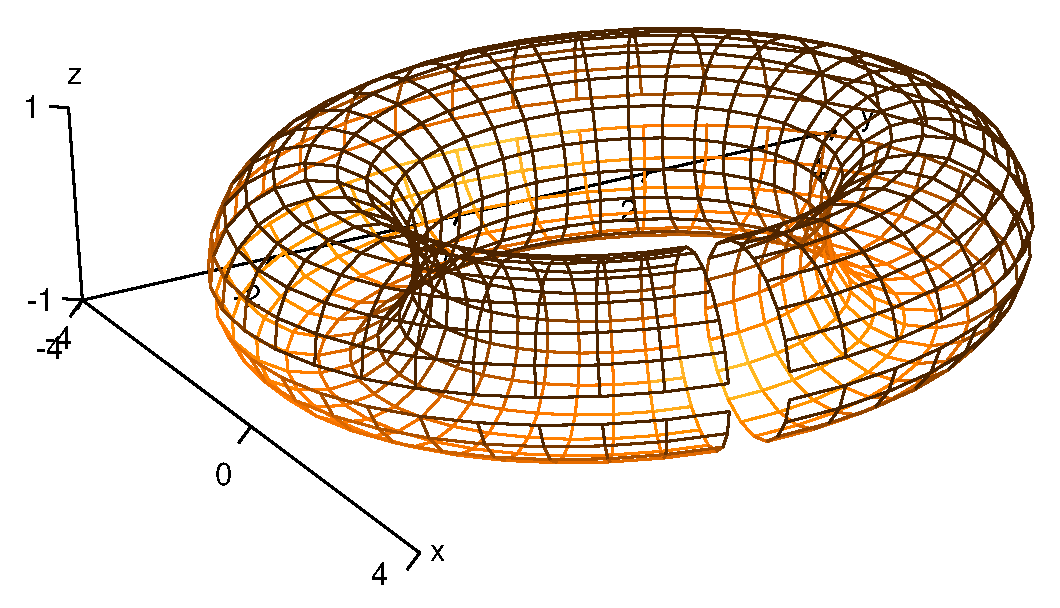
\includegraphics[width=9cm]{torus.eps}}

Closing the torus in the cumbersome manner shown in paragraph \numb section 2.\numb parag 14
is possible but not practical.
Paragraph \numb section 5.\numb parag 6 shows a more elegant solution.

If we only want a visual illusion of a closed surface, we may use the code below

\verbatim
   Cell A ( tag::vertex );  alpha(A) = 0.;     beta(A) = 0.;
   Cell B ( tag::vertex );  alpha(B) = 0.;     beta(B) = 2.*pi;
   Cell C ( tag::vertex );  alpha(C) = 2.*pi;  beta(C) = 2.*pi;
   Cell D ( tag::vertex );  alpha(D) = 2.*pi;  beta(D) = 0.;
   Mesh AB ( tag::segment, A.reverse(), B, tag::divided_in, 20 );
   Mesh BC ( tag::segment, B.reverse(), C, tag::divided_in, 40 );
   Mesh CD ( tag::segment, C.reverse(), D, tag::divided_in, 20 );
   Mesh DA ( tag::segment, D.reverse(), A, tag::divided_in, 40 );
   // AB, BC, CD and DA look like closed circles
   Mesh ABCD ( tag::rectangle, AB, BC, CD, DA );
   // ABCD gives the illusion of a closed torus
\endverbatim


\paragraph{\numb section 2.\numb parag 16. Starting with a high-dimensional manifold}

Instead of starting with a manifold having only the parameter(s), we may start with a
high-dimensional manifold containing both the geometric coordinates and the parameter(s),
then define the parametrization through equation(s).
% The advantage of this approach is that we can later shwitch on and off a constraint,
% thus switching between meshes of different dimensions.
There is a disadvantage however, regarding performance; see paragraph \dots

\verbatim
   Manifold RR5 ( tag::Euclid, tag::of_dim, 5 );
   Function xyzab = RR5.build_coordinate_system ( tag::Lagrange, tag::of_degree, 1 );

   // extract components of xyzab :
   Function x = xyzab[0], y = xyzab[1], z = xyzab[2], alpha = xyzab[3], beta = xyzab[4];

   // define a torus as a submanifold of RR5 :
   const double big_radius = 3, small_radius = 1;
   Manifold torus = RR5.parametric
      ( x == ( big_radius + small_radius * cos(beta) ) * cos(alpha),
        y == ( big_radius + small_radius * cos(beta) ) * sin(alpha),
        z == small_radius * sin(beta)                                );

   // define four corners
   const double pi = 3.1415926536;
   Cell A ( tag::vertex );  alpha(A) = 0.;       beta(A) = 0.;       torus.project(A);
   Cell B ( tag::vertex );  alpha(B) = 0.;       beta(B) = 1.9*pi;   torus.project(B);
   Cell C ( tag::vertex );  alpha(C) = 1.95*pi;  beta(C) = 1.9*pi;   torus.project(C);
   Cell D ( tag::vertex );  alpha(D) = 1.95*pi;  beta(D) = 0.;       torus.project(D);
   // four almost-closed circles :
   Mesh AB ( tag::segment, A.reverse(), B, tag::divided_in, 19 );
   Mesh BC ( tag::segment, B.reverse(), C, tag::divided_in, 39 );
   Mesh CD ( tag::segment, C.reverse(), D, tag::divided_in, 19 );
   Mesh DA ( tag::segment, D.reverse(), A, tag::divided_in, 39 );
   // build a rectangle
   Mesh ABCD ( tag::rectangle, AB, BC, CD, DA );  // an almost-closed torus

   // forget about alpha and beta :
   torus.set_coordinates ( x && y && z );
   // in future statements (e.g. for graphical representation)
   // x, y and z will be used, not alpha nor beta :
   ABCD.export_msh ("torus.msh");
\endverbatim

The {\codett Manifold::parametric} method is similar to {\codett Manifold::implicit}, presented in
paragraphs \numb section 2.\numb parag 3 -- \numb section 2.\numb parag 12.
The only difference is that by using {\codett parametric} we declare an explicit dependence%
\footnote *{\parbox{\ftntfont\baselineskip=3pt
Perhaps {\ftnttt explicit} would be a better name than {\ftnttt parametric};
unfortunately, that word is reserved in {\codett C++}.}}
of the coordinates (here, {\codett x}, {\codett y} and {\codett z}) upon the parameters
(here, {\codett alpha} and {\codett beta}).
This endows the manifold {\codett torus} with a different projection operator.
The projection of a vertex from {\codett RR5} onto {\codett torus} is done by merely updating
the values of {\codett x}, {\codett y} and {\codett z}, while keeping {\codett alpha} and
{\codett beta} constant.
